
\chapter{Enhancing human-robot physical collaboration with polytopes}


\todos{
\begin{itemize}
    \item last two chapters introduced the humans and robots physical abilities and their polytope form
    \item and how to solve them 
    \items this chapter proposes several use-cases of these metrics for real time robot control in collaborative scenarios
    \items First the \Cref{ch:motivation_collaborative_workstation} brings the general motivation of using the physical ability metrics and polytopes especially for enhancing human-robot physical collaboration
    \item then the \Cref{ch:collaborative_carrying} brings the example of the collaborative task requiring physical interaction and proposes two different control strategies which exploit the physical abilities of humans and robots 
    \item last section proposes something else, I don't know what exactly yet
\end{itemize}
}

\section{Motivation: Collaborative Workstation}
\label{ch:motivation_collaborative_workstation}
The industry of the future, as described by the movement called Industry 5.0~\cite{MADDIKUNTA2022ind50}, promises to step away from the traditional point of view on industrial automation, where the goal is to blindly automatise, as much processes as possible, in order to improve the overall efficiency and reduce the cost. The Industry 5.0 puts the human workers in the central position and aims to create the workflows that ensure their well-being as well as the long term sustainability of the industrial practices in general~\cite{XU2021ind50}. The industry of the future relies on the flexibility and adaptability of the human workers, by embracing their cognitive and physical skills as well as their talents and different levels of expertise. The role of the automation is no longer purely optimisation of the industrial processes, but providing the support and assistance to the human operator with the aim to exploit both machines' and humans' full potential, establishing human-automation symbiosis~\cite{LENG2022ind50} on the industry floor.
 
One typical example of such symbiosis is an industrial workstation~\cite{SIMOES2022workplace}, where the human and the robot work in a close proximity and interact physically to execute different tasks. The aim of such collaboration is to improve the overall efficiency by exploiting the abilities of both humans (flexibility, adaptability, cognitive capacity, expertise, etc.) and robots (repeatability, precision, tirelessness, etc.), as well as to improve the operators well-being, remove the unnecessary strain and ensure his safety when executing tasks. Therefore, such future collaborative scenarios require having a set of tools for characterising different abilities of robots and humans, as well as different notions of human well-being and safety. Such tools are required both for assessing different tasks and allocating them with respect to humans and robots abilities as well as for creating more human-centred robot control strategies.

%\todos{I'm more or less happy till here}

Even though human-robot collaboration is still relatively recent field, there are numerous performance metrics proposed in the literature that quantify different aspects of the quality of their collaboration and their individual abilities~\cite{CORONADO2022collab_quality}.
The main focus of this work is put on different tools for characterising human's and robot's physical abilities, especially their polytope representations, which have a great potential to be used in this context, both in order to quantify and leverage their individual abilities as well as to ensure human safety. As discussed in \Cref{ch:poly_metrics}, the polytope characterisations of different physical abilities are an accurate representations of physical abilities for both robots and humans. Furthermore, the polytopes enable expressing their individual physical abilities, as well as their joint physical abilities when collaborating, in the same polytope form. Such unified view on their capacities lays foundation for creating new task allocation strategies that take in consideration their physical abilities, by being able to asses if different tasks better suite human's or robot's abilities or potentially require their collaboration. 

Furthermore, both human's and robot's physical abilities are state dependant and can vary significantly during the task execution, and polytopes enable capturing the changes in their abilities as well. Having an accurate information about the robot's physical abilities online, enables creating robot control strategies that adapt to the their changes and exploit the robot's full potential. On the other hand, having an accurate online information about the human's physical abilities is important for assessing if the operator is apt to execute a certain task and quantifying if the operator needs assistance of the robot due to its lacking physical abilities. Furthermore, having the real-time information about the operator's physical abilities enables ensuring that his abilities are never surpassed which has a direct impact on the operator's safety and well-being. Therefore, the collaborative workstations require creating more human-centred robot control strategies where the robot adapts its behaviour not just with respect to the requirements of the task and its own abilities, but also to the current abilities of the human operator as well as his safety. As polytope characterisations of robot's and human's physical abilities can be easily integrated with different robot control strategies, they have a great potential to be used for creating such adaptive collaboration scenarios.

%\todos{more or less happy.}

This chapter presents the benefits of using the polytope based physical ability characterisations for creating real-time robot control strategies that enable such flexible collaboration scenarios. \Cref{ch:collaborative_carrying} brings an example of the task of collaborative object carrying within the collaborative workstation, where two collaborative scenarios are proposed. First scenario, introduced in \Cref{ch:robot_robot_carrying}, consists in two robots collaborating to carry a heavy object while the control strategies of each one of the robots take in consideration both their own and the other robot's physical abilities. Second scenario, proposed in \Cref{ch:human_robot_carrying}, consists in the human operator and the robot collaboratively carrying a heavy object, where the robot's control strategy takes in consideration its own physical abilities and the physical abilities of the operator in the real-time. 

\todos{
Furthermore, an assistive and human-centred robot control strategy that exploits the polytope geometry is described in section after.
}

\section{Collaborative carrying of a heavy object}
\label{ch:collaborative_carrying}

\begin{figure}[!h]
    \centering
    \includegraphics[width=0.8\linewidth]{Papers/images/carrying_schema.pdf}
    \caption{}
    \label{fig:carrying_schema}
\end{figure}

One traditional example of a collaborative task requiring physical interaction between multiple actors (humans and robots) is collaborative object carrying~\cite{Arai2000carrying,Kosuge1997carrying,Tsumugiwa2002carrying}. In this task $N$ actors collaborate physically by applying forces $\bm{f}_{a_i}$ on the object with mass $m$, in order to compensate for its gravity $G$
\begin{equation}
    G=m\bm{g}=\bm{f}_{a_1} + ~\cdots ~+\bm{f}_{a_N}
\end{equation}
An illustration of the human-robot and dual robot arm collaborative carrying is given on \Cref{fig:carrying_schema}. 

As discussed in \Cref{ch:collab_metrics}, in this particular collaboration scenario, each of the actors' capacity to generate forces $\bm{f}_{a_i}$ can be expressed in the polytope form
\begin{equation}
    \bm{f}_{a_i} \in \mathcal{P}_{f,a_i}
\end{equation}
while their joint capacity of generating the forces on the object can be found as the Minkowski sum of their polytopes
\begin{equation}
    \mathcal{P}_f = \mathcal{P}_{f,a_1} \oplus~\cdots~\oplus \mathcal{P}_{f,a_N}
\end{equation}
Therefore if the force of gravity of the object $G$ is within the polytope $\mathcal{P}_f$ the collaborative system is able to compensate for the objects weight
\begin{equation}
    G \in \mathcal{P}_f
\end{equation}

As both human's and robot's force capacity is state dependant and changes during the execution of the task, the role of the robot control strategies is to find the suitable forces $\bm{f}_{a_i}$ that respect their individual capacities $\mathcal{P}_{f,a_i}$ and accomplish the task by compensating the objects weight $G$. 

The following two sections present two different robot control strategies for two different collaborative object carrying scenarios. \Cref{ch:robot_robot_carrying} brings a physical collaboration scenario based on two robotic arms carrying an object with a mass of 12kg. Their physical abilities are calculated in real-time in the polytope form and integrated in the real-time robot control in order to exploit their full force capacity. \Cref{ch:human_robot_carrying}, on the other hand, proposes the human-robot physical collaboration scenario for carrying of an object with the mass of 7kg. In this scenario, both of their physical abilities are evaluated online and used to create a human-centred robot control strategy, able to exploit their changing physical abilities while ensuring operators safety, by verifying that his physical abilities are not surpassed. 


\subsection{Dual robotic arm collaborative object carrying}
\label{ch:robot_robot_carrying}

\begin{figure}[!h]
    \centering
    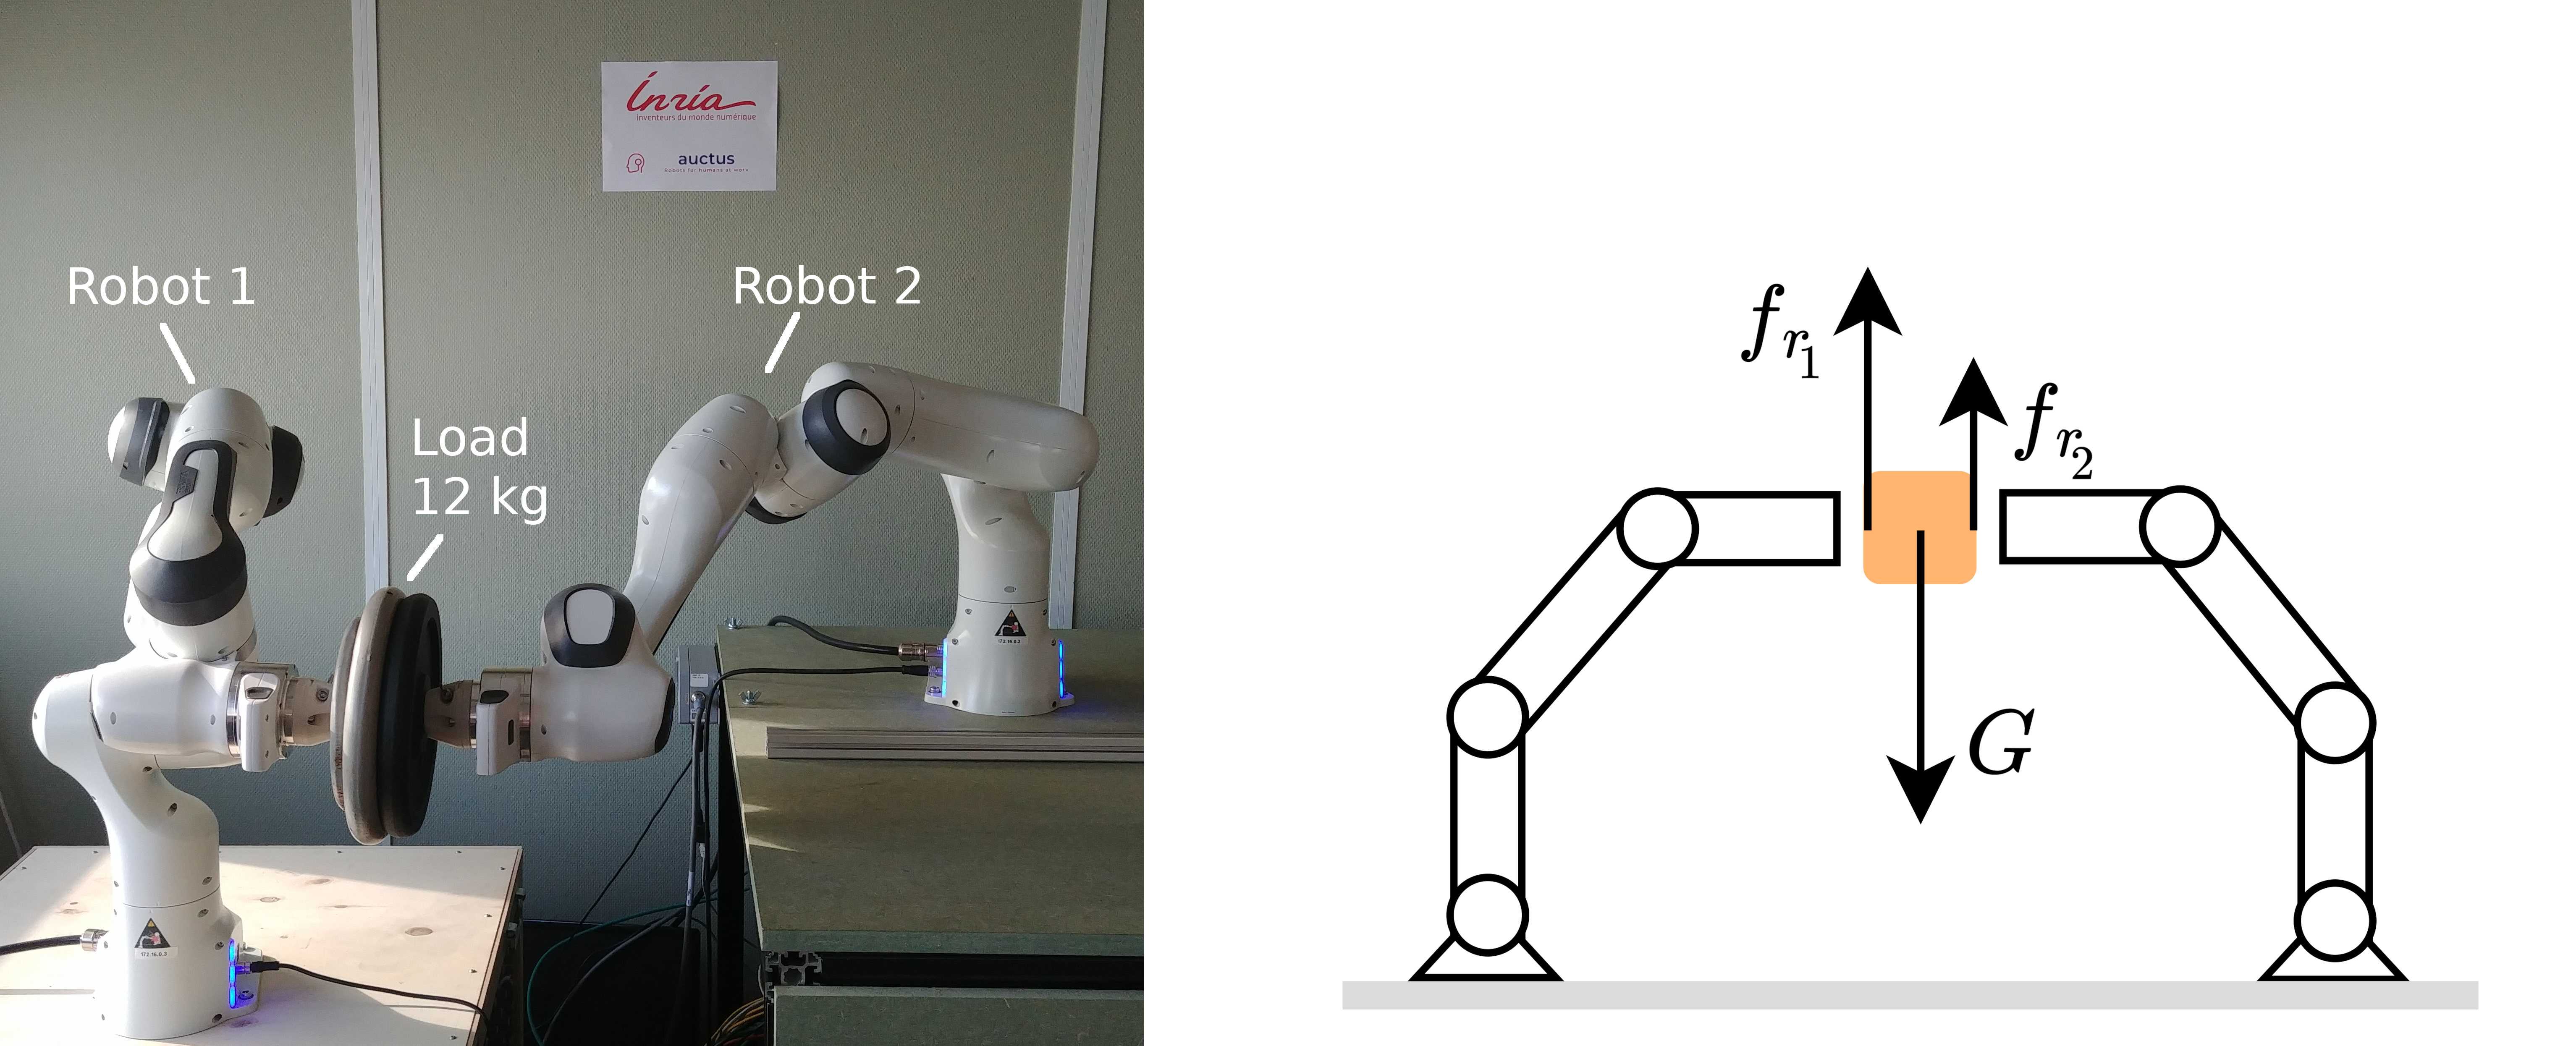
\includegraphics[width=\linewidth]{Papers/images/real_robots_schema_exp1.png}
    \caption{}
    \label{fig:exp1_real_schema}
\end{figure}


This sections presents a physical collaboration scenario using two \textit{Franka Emika Panda} robots involved in a collaborative load carrying task for an object of mass $m$. Each robot is contributing to the compensation of the overall gravity force $G=m\bm{g}$ applied at the end-effector by the carried object, with forces $\bm{f}_{r_1}$ and $\bm{f}_{r_2}$ respectively such that
\begin{equation}
    \bm{f}_{r_1} + \bm{f}_{r_2} = G
\end{equation}

Panda robots are rated to a maximal carrying capacity of 3kg which corresponds to the absolute minimal carrying capacity of the robot evaluated in one of its near-singular configurations. It is, by definition, an underestimation of the real robot task space wrench capacity and relying on it, as it is commonly done, limits the scope of the possible tasks and applications.

The goal of this experiment is to demonstrate the fact that by taking into account the true force capabilities of each robot, it is possible to go considerably beyond the robot's conservative rated capacity without comprising safety nor exceeding any of the actuation limits. The weight of the object chosen for the experiments is $m=12kg$, voluntarily far above the recommended joint carrying capacity $ m\le 6kg$. 

The following \Cref{sec:robot_carrying_capacity} proposes an efficient approach for calculating the carrying capacity of both robots, while \Cref{sec:collab_robot_control_double_robot} proposes a robot control strategy exporting this real time information in order to fully exploit the real-time changes in their capacity. Finally, \Cref{sec:experiment_dual_robto_carrying} brings the experimental validation of the approach, as well as the discussion of the results. 

\subsubsection{Robot carrying capacity calculation}
\label{sec:robot_carrying_capacity}


As the carrying task requires the robots to apply only the forces $f_{r_1}$ and $f_{r_2}$ that are opposite to the force of the object's gravity $G$, their physical ability to carry certain weight can be evaluated as the maximal applicable force in the vertical ($z$-axis) direction. Therefore, the robot's carrying capacity $\mathcal{F}_z$ can be expressed as the the special case of the robot's wrench polytope $\mathcal{P}_{f}$, described in \Cref{ch:poly_force}, where the task space is one dimensional ($m=1$)
\begin{equation}
    \mathcal{F}_z (\bm{q},\dot{\bm{q}}) = \mathcal{P}_{f_z} (\bm{q},\dot{\bm{q}}) = \{ f \in \mathbb{R} ~|~ J_{z}(\bm{q})^Tf=\bm{\tau} - \bm{\tau}_b(\bm{q},\dot{\bm{q}}), \quad \bm{\tau}\in[\bm{\tau}_{min}, ~\bm{\tau}_{max}]\}
\end{equation}

where $\{\bm{q},\dot{\bm{q}}\}$ represent the robot's joint state, $f \in\mathbb{R}$ is the applicable scalar force in $z$-axis direction, $\bm{\tau}\in\mathbb{R}^n$ are the applied joint torques limited within the interval $\bm{\tau}\in[\bm{\tau}_{min}, ~\bm{\tau}_{max}]$, the $\bm{\tau}_{b}\in\mathbb{R}^n$ represents the bias joint torques grouping the effects of the gravity and robot's motions, while $J_{z}\in\mathbb{R}^{1\times n}$ is the state dependant jacobian matrix with one line and $n$ columns.

Geometrically, the $m=1$ dimensional polytope, describing the range of scalar forces $f$ in applicable the vertical direction, can be represented as the intersection of the complete wrench/force ($m=6$/$m=3$) polytope $\mathcal{P}_f$, described in \Cref{ch:poly_force}, with the vertical axis. An illustrative view of this intersection is shown on \Cref{fig:carrying_cap_robot}.

\begin{wrapfigure}{r}{0.35\linewidth}
    \centering
    \includegraphics[width=\linewidth]{Papers/images/carrying_capacity_robot.pdf}
    \caption{}
    \label{fig:carrying_cap_robot}
\end{wrapfigure}

For any given robot state $\{\bm{q},\dot{\bm{q}}\}$ this one dimensional set $\mathcal{F}_z$ can be transformed into the form of a min-max interval
\begin{equation}
    \mathcal{F}_z = \{ f \in \mathbb{R} ~|~ f \in[{f}_{min}, ~{f}_{max}]\}
\end{equation}
Finding the limits $[f_{min},~f_{max}]$ of the applicable scalar force $f$ in the vertical direction can be viewed as finding a $\repr{V}$-representation of the 1D ($m=1$) polytope $\mathcal{F}_z$. Then the vertex search algorithm described in \Cref{sec:algorithm_vea} can be used to efficiently find the limits (vertices) $f_{min}$ and $f_{max}$ of the applicable force in $z$-axis direction.  

Furthermore, this procedure can be done for both robots $r_1$ and $r_2$, by characterising their carrying capacities
 $\mathcal{F}_{z,r_1}$ and $\mathcal{F}_{z,r_2}$ and finding their applicable vertical force ranges 
\begin{equation}
    f_{r_1} \in [f_{r_1,min}, ~f_{r_1,max} ], \quad f_{r_2}\in [f_{r_2,min}, ~f_{r_2,max}]
    \label{eq:robot_robot_carrying_capacity}
\end{equation}
 
Additionally, their combined carrying capacity $\mathcal{F}_{z,r_1+r_2}$ can be calculated as the Minkowski sum of their polytopes $\mathcal{F}_{z,r_1}$ and $\mathcal{F}_{z,r_2}$ 
$$\mathcal{F}_{z,r_1+r_2} = \mathcal{F}_{z,r_1}\oplus \mathcal{F}_{z,r_2}$$
or in this special ($m=1$), the sum of the intervals 
$$f_{r_1+r_2} = f_{r_1}+f_{r_2} \in  [f_{r_1,min} + f_{r_2,min}, ~f_{r_1,max} + f_{r_2,max}].$$


\subsubsection{Collaborative robot control strategy}
\label{sec:collab_robot_control_double_robot}
The collaborative carrying task requires the robot's to apply forces that combined compensate for the object's weight $G$ 
$$f_{r_1} + f_{r_2} = G$$

To efficiently distribute and adapt the carried load between the robots, while making sure that their carrying capacity is not exceeded, a robot control strategy based on Quadratic Programming (QP) is proposed
\begin{equation}
\begin{split}
    \min_{f_{r_1},f_{r_2}} &~\overbrace{||G - f_{r_1} -f_{r_2}||^2}^{\text{weight compensation}} ~~+ \overbrace{\omega \lambda_1||f_{r_1}||^2 + \omega \lambda_2||f_{r_1}||^2}^{\text{weight distribution}}\\
    s.t.& \quad f_{r_1} \in[f_{r_1,min}, f_{r_1,max}]\\
    & \quad f_{r_2} \in[f_{r_1,min}, f_{r_2,max}]\\
\end{split}
\label{eq:qp_robot_robot}
\end{equation}
The main component of the cost function of this optimisation problem is the minimisation of the error $||G - f_{r_1} -f_{r_2}||^2$ ensures that the object's gravity is always compensates, as long as their carrying capacity defined in the constraints of the optimisation problem allows for it. 

Finally, two additional regularisation components of the cost function are added to minimise the magnitude of both forces $f_{r_1}$ and $f_{r_2}$. In order to allow for an efficient distribution of the load between the robots, their forces are not weighed equally, but using the factors $\lambda_1$ and $\lambda_2$ corresponds to the ratios of their contribution to the overall carrying capacity 
\begin{equation}
\lambda_1 = \frac{f_{r_2,max}}{f_{r_1,max} + f_{r_2,max}}, \qquad \lambda_2 = 1- \lambda_1
\end{equation}

For example, if the robot $r_1$ has much higher carrying capacity $f_{r_1,max}\gg f_{r_2,max}$ than the robot $r_2$, then $\lambda_2\gg\lambda_1$,  meaning that the force $f_{r_2}$ is going to be weighed (penalised) much more in the cost function, ultimately resulting in much lower optimal values found by the QP algorithm. On the other hand, if the carrying capacities of both robots is equal, then the weighing factors are equal too $\lambda_1=\lambda_2$, resulting in the equal weight distribution.  

The regularisation factor $\omega$ is used to set the priority of the weight distribution task much lower than the main task of the weight compensation of the object, in the experiments proposed in this sections the regularisation weight is set to $\omega=1\times 10^{-5}$.

Each robot control cycle starts by calculating the carrying capacity of both robots (\ref{eq:robot_robot_carrying_capacity}), followed by the resolution of the optimisation problem (\ref{eq:qp_robot_robot}). Once the optimal vertical forces $f_{r_i}$ are obtained the joint torques $\bm{\tau}_{r_i}$, achieving those forces, are calculated for each of the robots and sent to their low-level joint controllers 
\begin{equation}
    \bm{\tau}_{r_i} = J_{z,r_i}^T(\bm{q}_{r_i}){f}_{r_i} - \bm{\tau}_{b,r_i}(\bm{q}_{r_i},\dot{\bm{q}}_{r_i}), \qquad \forall i \in \{1,2\}
\end{equation}

\subsubsection{Experimental validation}
\label{sec:experiment_dual_robto_carrying}
\begin{figure}[!h]
    \centering
    \includegraphics[width=\linewidth]{Papers/images/exp1_explication.png}
    \caption{}
    \label{fig:experiment1}
\end{figure}

In this experiment, a human operator is moving the object freely through the common work-space, implicitly changing both robots positions and configurations in real-time. As a consequence, the task space trajectory and the evolution of the robot configurations are not known in advance. The particular trajectory taken by the human operator in this experiment is indicated on \Cref{fig:experiment1}. 
The trajectory executed by the operator consisted in taking the load through the common work-space making a forward and backward pass through four via-points. The robots calculated the changes in their carrying capacity in real-time and adapted the weight distribution to their varying physical abilities, in order to ensure the object's weight compensation during the whole experiment. 

\qrimg{qrcodes/icra2021.png}{https://youtu.be/hApIv1oFuhk}{Video}
A straightforward control strategy, requiring each robot to compensate for half of object mass $f_{r_1}=f_{r_1}=0.5G$ is taken as baseline to evaluate the performance of the new method.

Furthermore, the experiment has been implemented using the Robot Operating System (ROS) programming environment. Both robots are torque controlled at the frequency of 1kHz. The update of the carrying capacity calculations are performed at 40Hz and implemented in programming language Python. All the control software is run from one computer with the 1.90GHz Intel i7-8650U processor. 
This experiment is illustrated in the accompanying video\footnote{https://youtu.be/hApIv1oFuhk}.

\begin{landscape}
\begin{figure}
    \centering
    \includegraphics[width=\linewidth]{Papers/images/exp_no_anim.jpg}
    \caption{This figure shows the time evolution of different control and physical ability variables in the top graphs, as well as several images of the experiment taken when the operator attained different via-points with the object. 
   The top graph shows the time evolution of the carrying capacity of the manipulators $f_{r_1,max},f_{r_2,max}$, indicating, with red background, the time periods when the naive strategy $f_{r_1}=f_{r_2}=0.5G$ (dashed line on all graphs) would not be feasible for at least one of the two robot. 
   The second  graph provides the evolution of their joint capacity $f_{max}=f_{r_1,max}+f_{r_2,max}$, indicating their individual contributions to the common capacity. The third graph indicates the time evolution of applied manipulator forces $f_{r_1}, f_{r_2}$, calculated using the proposed control strategy. Finally, the bottom graph shows the time evolution the weights $\lambda_1,\lambda_2$ used with the robot control. All the force values are expressed in kilograms for easier readability.     
    }
    \label{fig:dual_manip}
\end{figure}
\end{landscape}

\Cref{fig:dual_manip} (bottom) shows several images taken during the experiment execution in the moments when the operator reached different via-points, while the graphs on the top show the time evolution of the evaluated maximal forces and force applied by each robot during the experiment. Additionally, the naive strategy $f_{r_1}=f_{r_1}=0.5G$ is shown in dashed lines for comparison. 

The results show that the proposed control strategy is successful in ensuring compensation of the object weight during the full length of the experiment. In the starting via-point $t=0$s and $t\geq21$s, robot $r_2$ (robot on the right) is close to it's singular configuration and its load carrying capacity is close to $5$kg. Controlling it to compensate for half of the weight of the object would result in a security exception and could damage the robot hardware. The same is true for via-point 4 at $t=12$s. In this via-point the robot $r_1$ (robot on the left) is not be able to compensate for half of the object weight but thanks to the proposed adaptive control law, the task can successfully be achieved. 
Furthermore, any naive fixed strategy, assigning certain fixed ratio of the objects weight to the robots, would resulted in surpassing robots' limits and would not be be able to accomplish this task. By exploiting the online calculation of the robots' physical abilities, the proposed strategy was able to exploit their changing abilities and enable accomplishing this task while at the same time guaranteeing that their capacities are not exceeded.

The results further show that even though in the large portion of the experiment one of the robots was not able to carry half of the object's weight, their joint carrying capacity exceeded the objects weight $f_{r_1,max}+f_{r_2,max} >G$ during the whole length of the experiment. 

However, this may not be the case over the entire common workspace of the two robots, but this example is a good illustration of the interest of accounting for the true capabilities of the system at the control level.  In certain configurations the common carrying capacity of the robots might be lower than the objects weight $f_{r_1,max}+f_{r_2,max} <G$. The proposed control approach, in those cases would still be able to ensure that the robot's physical abilities are not exceeded, however it would not be able to guarantee the weight compensation of the object. 



\subsection{Human-robot collaborative object carrying}
\label{ch:human_robot_carrying}

This section brings an example scenario of the human-robot physical collaboration in order to execute the task of the carrying and manipulation of a heavy object, common in the industrial assembly procedures. In this scenario, shown on \Cref{fig:exp2_real_schema}, a human operator and a \textit{Franka Emika Panda} robot jointly carry $m\!=\!7$ kg object, each one compensating for a part of the total weight 
\begin{equation}
    \bm{f}_h  + \bm{f}_r = m\bm{g} = G
\end{equation}

\begin{figure}[!t]
    \centering
    \includegraphics[width=\linewidth]{Papers/images/exp2_real_schema.jpg}
    \caption{}
    \label{fig:exp2_real_schema}
\end{figure}

This scenario is inspired by common industrial tasks requiring 
the manipulation of a heavy object. The operator has the expert knowledge about the task and moves the object through the workspace to perform the task efficiently. The robot's role, in this case, is to assists the operator with the carrying of the heavy object and improve his well-being.

The usual choice for these scenarios is a simple gravity compensation strategy, making the robot carry the full weight of the object $\bm{f}_r = G$ and provide the operator with full movement transparency. Several human-centred robot control strategies have recently been proposed in the literature, where the robot in addition to the full weight compensation improves different aspects of the human safety and ergonomics. One example of such approach is proposed by \citet{ferraguti2020unified}, which REBA \cite{reba} ergonomic indicators to improve human posture while carrying an object. 

However, as discussed in previous section, \Cref{ch:robot_robot_carrying}, assigning any fixed weight to the robotic manipulator requires \textit{a priori} analysis of its changing capacity and determination of the \textit{worst-case} weight limits, which in the case of the Franka Emika Panda robot is $m\leq3$kg\footnote{Given by the manufacturer in the form of the robot's rated payload.}. Therefore, carrying the 7kg load requires using a more capable robot which, in many cases, significantly increase the cost of such system and potentially reduces operator's safety. More capable robots are usually bigger and heavier, which in case of impact with the operator, results in higher exchanged forces~\cite{smu}.
Therefore, delegating the entire weight compensation to the robot is not always be the most efficient or the safest solution for the operator. 

On the other hand, several studies have shown that the human's physical feedback during task execution improves significantly his engagement in the task \cite{rani2007operator}, improves the task execution efficiency and reduces the risk of the human error \cite{BYRNE1996249}. However, since the human's carrying capacity varies significantly throughout the workspace as well, before allocating any weight to the operator, his safety has to be ensured. As in the case of robots, the traditional approach consists in analysing the task in advance and determining, often very conservative, the set of \textit{worst-case} limits \cite{shoaf1997comprehensive}, often given in a form of different standards \cite{nasa} and manuals \cite{health1992manual}. 

In order to avoid making such coarse assumptions, several approaches have been proposed in the literature, able to quantify different measures of human physical abilities and adapt the human load to their changes online. \citet{Kim2018} have proposed an approach estimating the joint torques in the operator's body produced by carrying the load of the object, where the robot role is to adapt his posture to minimise necessary torques. In their work, the human body was approximated using a planar model actuated at the joint level. In their work however, human was the one carrying the full mass of the object, while the only role of the robot was modify the operator's posture in order to improve his ergonomics.

A different approach was proposed by \citet{carmichael2013admittance}, where the authors used a more accurate human model based on human musculoskeletal models. This approach uses an efficient approximation of the human's force capacity to modulate the weight carried by the human with respect to his changing abilities. This work is developed in the context of human rehabilitation and used for the real-time control of assistive exoskeletons, where the authors showed that such approach is capable of adapting to the operators pathology and reduce the rehabilitation time~\cite{Carmichael2013Experimental}. 
This work shows the potential of using human-centred robot control strategies which are able to adapt the load carried by the human precisely to his varying physical abilities. However due to the intractable computational complexity of the human force capacity calculation proposed by the authors, the scope of their work is limited to relatively simple planar musculoskeletal models. Furthermore, the robot control strategy proposed in their work is aimed to the rehabilitation and the use of assistive exoskeletons, which does not transpose well to more unstructured industrial scenarios.

Inspired by their work, this section aims to further demonstrate the potential of using the real-time knowledge about both robot's and human's physical abilities in the context of collaborative robot control in industrial scenarios. The proposed collaborative robot control strategy leverages the two new algorithms developed in the context of this work, capable of efficiently calculating the force capacity of robots (\Cref{sec:algorithm_vea}) and humans, based on their musculoskeletal models (\Cref{ch:algorihtm_ichm}). 
Their changing capacities are calculated online and used to create collaborative robot control strategy, capable of both exploiting their full potential and, at the same time, ensure the safety of the operator. 

\Cref{sec:human_carrying_capacity} introduces an efficient strategy of calculating the operators carrying capacity in real-time. \Cref{sec:collab_robot_control_human_robot} the introduces the collaborative robot control strategy using the online information about the operator's carrying capacity as well as the robot's capacity, described in  \Cref{sec:robot_carrying_capacity}. The experimental validation of this approach is described in  \Cref{sec:human_robot_experiment}, followed by the discussion on prospective applications and limitations in  \Cref{sec:human_robot_prospective}.


\subsubsection{Human carrying capacity calculation}
\label{sec:human_carrying_capacity}

Assuming that the musculoskeletal model of the operator is available, this model can be used to evaluate different physical abilities of the operator. Some of the most common physical abilities in the literature are listed in \Cref{ch:human_metrics}. 

When it comes to the collaborative carrying experiment, the operator is required to apply only the force $f_{h}$ that contributes to compensating the object's gravity $G$. Therefore, his task is effectively one dimensional $m=1$ and his physical ability to carry certain weight can be evaluated as the maximal applicable force in the vertical ($z$-axis) direction. Hence, the human's carrying capacity $\mathcal{F}_z$ can be expressed as the the special case of the human's wrench polytope $\mathcal{P}_{f}$, described in  \Cref{ch:force_poly_human}, where the task space is one dimensional ($m=1$)
\begin{equation}
     \mathcal{F}_z(\bm{q},\dot{\bm{q}}) = \mathcal{P}_{f_z} (\bm{q},\dot{\bm{q}}) = \{ f \in \mathbb{R} ~|~ J_{z}(\bm{q})^Tf=N(\bm{q})\bm{F} - \bm{\tau}_b(\bm{q},\dot{\bm{q}}), \quad \bm{F}\in[\bm{F}_{min}, ~\bm{F}_{max}]\}
\end{equation}
where $\{\bm{q},\dot{\bm{q}}\}$ represent the human's joint state, $f \in\mathbb{R}$ is the applicable scalar force in $z$-axis direction, $\bm{F}\in\mathbb{R}^n$ are the applied muscular forces limited within the interval $\bm{F}\in[\bm{F}_{min}, ~\bm{F}_{max}]$, the $\bm{\tau}_{b}\in\mathbb{R}^n$ represents the bias joint torques grouping the effects of the gravity and human's motions, while $J_{z}\in\mathbb{R}^{1\times n}$ is the state dependant jacobian matrix with one line and $n$ columns and $N\in\mathbb{R}^{n\times d}$ is the state dependant moment arm matrix. Values $n$ and $d$ correspond to the number of joints and muscles considered in the musculoskeleral model.


\begin{wrapfigure}{r}{0.4\linewidth}
    \centering
    \includegraphics[width=\linewidth]{Papers/images/carrying_capacity_human.pdf}
    \caption{}
    \label{fig:carrying_cap_human}
\end{wrapfigure}
Analogously to the robot's case, human's carrying capacity $\mathcal{F}_z$ is a $m=1$ dimensional polytope, describing the range of scalar forces $f$ applicable in the vertical direction. Geometrically, this polytope corresponds to the intersection of the complete wrench/force ($m=6$/$m=3$) polytope $\mathcal{P}_f$, described in \Cref{ch:force_poly_human}, with the vertical axis. An illustrative view of this intersection is shown on \Cref{fig:carrying_cap_human}.

Furthermore, for any given human's state $\{\bm{q},\dot{\bm{q}}\}$ this one dimensional set $\mathcal{F}_z$ can be transformed into the form of a min-max interval
\begin{equation}
    \mathcal{F}_z = \{ f \in \mathbb{R} ~|~ f \in[{f}_{min}, ~{f}_{max}]\}
\end{equation}
In order to find the limits $[f_{min},~f_{max}]$ of the applicable scalar force $f$ in the vertical direction, this problem can be formulated as finding the $\repr{V}$-representation of the 1D ($m=1$) polytope $\mathcal{F}_z$. Then the real-time capable algorithm, proposed in \Cref{sec:algorithm}, can then be used to find the limits (vertices) $f_{min}$ and $f_{max}$ of the applicable force in $z$-axis direction.  

Following the similar procedure as for humans, the robot's carrying capacity can be determined in real-time as well, as proposed in \Cref{sec:robot_carrying_capacity}. Then the human's carrying capacity $\mathcal{F}_{z,h}$ and robot's carrying capacity $\mathcal{F}_{z,r}$, characterising their feasible ranges of applicable vertical forces $f_r$ and $f_h$ can be expressed as in the form of ranges
\begin{equation}
    f_{h}\in [f_{h,min}, ~f_{h,max}], \qquad f_{r} \in [f_{r,min}, ~f_{r,max} ]
    \label{eq:human_robot_carrying_capacity}
\end{equation}

Additionally, their combined carrying capacity $\mathcal{F}_{z,h+r}$ can be calculated as the Minkowski sum of their carrying capacities $\mathcal{F}_{z,h}$ and $\mathcal{F}_{z,r}$ 
$$\mathcal{F}_{z,h+r} = \mathcal{F}_{z,h}\oplus \mathcal{F}_{z,r}$$
or in this special ($m=1$), the sum of the intervals 
$$f_{h+r} = f_{h}+f_{r} \in  [f_{h,min} + f_{r,min}, ~f_{h,max} + f_{r,max}].$$

\subsubsection{Collaborative robot control strategy}
\label{sec:collab_robot_control_human_robot}

The collaborative carrying task requires the human and the robot to apply forces that combined compensate for the object's weight $G$ 
$$f_{h} + f_{r} = G$$
As their carrying capacity changes in time, the main task of the robot's control algorithm consists in modulating the weight carried by the operator and the robot to ensure that their carrying capacity is not exceed while compensating for the object's weight.

In addition to the object's weight compensation, inspired by the Assist-As-Needed (AAN) paradigm proposed by 
\citet{carmichael2013admittance}, a simple adaptive weight distribution strategy is proposed, with the goal to ensure that the human operator's relative load remains constant with respect to its real-time capacity. The fixed ratio chosen for the experiments is 30\% of the human's carrying capacity, ensuring operator's safety and maintaining the constant level of engagement.
$$
f_h = 0.3 f_{h,max}
$$

The main task of the object's weight compensation as well as the AAN strategy, maintaining the constant relative load of the operator, is implemented in a single robot control strategy based on Quadratic Programming (QP)
\begin{equation}
\begin{split}
    \min_{f_r,f_h} &~\overbrace{||G - f_r -f_h||^2}^{\text{weight compensation}} ~~+ \overbrace{\omega||f_r||^2}^{\text{weight distribution}}\\
    s.t.& \quad f_h \in[0.3f_{h,min}, ~0.3f_{h,max}]\\
    & \quad f_r \in[f_{r,min}, ~f_{r,max}]\\
\end{split}
\label{eq:qp_human_robot}
\end{equation}
The main component of the cost function of this QP is the minimisation of the error $||G - f_{h} -f_{r}||^2$, which ensures that the object's gravity is always compensates, as long as their carrying capacity defined in the constraints of the optimisation problem allows for it. 

The Assist-As-Needed (AAN) strategy is formulated as a regularisation task $\omega||f_r||^2$ in the cost function. This task minimises the magnitude of force $f_{r}$ applied by the robot while having no penalisation for the human's force $f_h$. The resulting behaviour of the optimisation problem is to find the weight distribution between the human and the robot which results in the minimal force $f_{r}$ applied by the robot, while maximising the force of the operator $f_h$. In the other words, this weight distribution strategy produces the AAN behaviour where the human applies its maximal forces (30\% of its carrying capacity) while the robot compensates for the rest. More precisely, the force the human applies is equal either to 30\% of its carrying capacity or the full objects weight
$$
f_h = \begin{cases}
    0.3f_{h,max},& \text{if } G\geq 0.3f_{h,max}\\
    G,              & \text{otherwise}
\end{cases}
$$
while the robot applies carries the remaining weight, as long as its capable of doing so
$$
f_r =  \begin{cases}
    G-f_h,& \text{if } G-f_h\geq f_{r,max}\\
    f_{r,max},              & \text{otherwise}
\end{cases}
$$

It is worth noting that if the object's weight exceeds the common carrying capacity of the robot and the operator $$f_{r,max} + 0.3f_{h,max} < G$$
they are not able to compensate for the weight of the object and the object will fall. 

The regularisation factor $\omega$ is used to set the priority of the AAN task lower than the main task of the weight compensation of the object, in the experiments proposed in this sections the regularisation weight is set to $\omega=1\times 10^{-2}$.

In each control cycle human's $\mathcal{F}_{z,h}$ and robot's $\mathcal{F}_{z,r}$ carrying capacities are calculated. These values are then used for the resolution of the optimisation problem (\ref{eq:qp_human_robot}). Once the robot's optimal vertical force $f_{r}$ is obtained, the joint torques $\bm{\tau}_{r}$ achieving this force are calculated using the expression
$$
\bm{\tau}_r = J_{z,r}^T(\bm{q}_r) f_r - \bm{\tau}_{b,r}(\bm{q}_r,\dot{\bm{q}}_r)
$$
where $\{\bm{q}_r,\dot{\bm{q}}_r\}\in \mathbb{R}^{n_r}$ is the robot's $n_r$ dimensional state, $J_r\in\mathbb{R}^{\times n_r}$ is the end-effector Jacobian with 1 line and $n_r$ columns, $\bm{\tau}_{b,r} \in\mathbb{R}^{n_r}$ is robot's torque vector corresponding to the effects of the gravity and the robot's motion and $\bm{\tau}_r \in\mathbb{R}^{n_r}$ are the joint torques sent to the robot's low-level joint control. 

\subsubsection{Experimental validation}
\label{sec:human_robot_experiment}

In this experiment, the human operator performs a task by {visually} navigating the object through the common workspace, passing through {the set of} 4 via-points. The object is fixed in the end-effector of the robot as well as at the hand of the human operator using a handle. \Cref{fig:experiment2} shows the experimental setup indicating the structure of the collaborative workstation, the placement of the via-points and the handle. 
The experiment is illustrated in the accompanying video\footnote{https://youtu.be/wg4E62AkNnM}.

\qrimg{qrcodes/icra2022.png}{https://youtu.be/wg4E62AkNnM}{Video}


The experiment is repeated two times, for two different operator positions, equally distant from the via-points, but rotated by 90° in space. These operator positions are indicated on \Cref{fig:experiment2} as well. Furthermore, in each of the two experiments, the operator performs 10 cycles through the via-points.


\begin{figure}[!t]
    \centering
    \includegraphics[width=\linewidth]{Papers/images/both_pose_explanation.jpg}
    \caption{{These figures show the experimental setup. The robot end-effector is fixed to the carried object and the human operator is holding the object by the handle. The motion capture system is used to acquire the pose of the human arm. The via-points are visually indicated to the human operator with numbered stickers on the table placed at the corners of a 30 cm square. The images shows the experiment 1 (left) and the experiment 2 (rigth).}}
    \label{fig:experiment2}
\end{figure}

\begin{wrapfigure}{r}{0.4\linewidth}
    \centering
    \includegraphics[width=\linewidth]{Papers/images/model_50m7dof.png}
    \caption{Caption}
    \label{fig:model_musc}
\end{wrapfigure}

The human upper limb configuration is inferred in real-time using an OptiTrack~\cite{optitrack} motion capture system. The musculoskeletal model analysis is developed using the efficient biomechanics library {biorbd} \cite{Michaud2021}. The musculoskeletal model used in this experiment is the 50 muscles, 7 degrees of freedom MOBL-ARMS model \cite{saul2015benchmarking}  developed by \citet{holzbaur2005model}. The visualisation of this model, using the biomechanics software Opensim \cite{opensim}, is shown on \Cref{fig:model_musc}.

The human subject (male, 182 cm, 80 kg) and the model belong to the same 50th percentile anthropomorphic group \cite{gordon1989anthropometric} so no model scaling \cite{correa20112782} is necessary.


Both robot's and human's carrying capacity calculation algorithms, as well as the robot control strategy described in \Cref{sec:collab_robot_control_human_robot}, are implemented in Python and run in real-time with the update frequency of 100Hz. The low-level robot control is implemented in C++, and run in real-time at the frequency of 1kHz. All the software components are integrated using the Robot Operating System (ROS) and run on a computer with 1.90GHz Intel i7-8650U processor. 

\Cref{fig:experiment_results} shows the recorded time evolution of robot's and human's carrying capacities and weight carried during the 10 cycles for each of the two experiments.

The figure shows (top graphs) that the human's carrying capacity is much more variable that the robot's one, peaking around 20kg in the recorded experiments and going as low as 5kg, emphasising the importance of measuring it in real-time. Furthermore, the experiment's show that the human's carrying capacity is in many cases much higher than the robot's capacity, confirming the importance of creating the control strategies able to account for both of their physical abilities. 

The second line of graphs on \Cref{fig:experiment_results} shows the time evolution of the sum of their carrying capacities, their carrying capacity as one system. The graphs show that even though both robot and the human, in multiple instances during the experiment runs, had carrying capacity lower than the object's weight $G$, their joint carrying capacity exceed the object's weight during the whole time of the experiment. Therefore, neither the operator or the robot would have been able to carry the object on their own, but by collaborating they were able to execute this task.

However, this may not be the case over the entire common workspace, but this example is a good illustration of the interest of accounting for the true capabilities of the system at the control level. In certain configurations the common carrying capacity of the human and the robot might be lower than the objects weight $f_{h,max}+f_{r,max} <G$. The proposed control approach, in those cases would still be able to ensure that both robot's and human's physical abilities are not exceeded, however it would not be able to guarantee the weight compensation of the object. 

The third line of graphs shows the time evolution of the weight carried by the robot and the human, while the bottom graphs on \Cref{fig:experiment_results}, show the carrying load of the robot $l_r$ and the human $l_h$ calculated as
$$
l_h = \frac{f_h}{f_{h,max}}, \qquad l_r = \frac{f_r}{f_{r,max}}
$$
The graphs confirm that the proposed control strategy maintained the human's relative load at 30\% ($l_h=0.3$) of its capacity as proposed by the Assist-As-Needed (AAN) strategy, while the robot's relative load $l_r$ depended on the human capacity. As the human's carrying capacity decreased robot's load $l_r$ increased, and \textit{vice-versa}. By having the real-time knowledge about the operator's carrying capacity, the robot was able to adapt its assistance level to maintain human's load constant, despite substantial changes in the operator's capacity profile and despite the his changing placement in the workspace. 

In summary, the experimental validation, presented in this section, demonstrates the benefits of integrating accurate real-time information about, both the human operator's and the robot's, physical abilities within the robot control strategy in the context of human-robot physical collaboration.

The proposed robot control strategy exploits both robot's and human's physical abilities, while guaranteeing that neither of their abilities is surpassed. As demonstrated in the experiments, even though their individual abilities are not suitable for executing this task on their own, by collaborating the task become feasible, as their combined abilities (as a single system) are higher than the requirements of the task. In addition to efficiently combining both operator's and robot's physical abilities, the proposed control strategy was able to further ensure safety and operator's engagement in the task, by modulated the weight carried by the human operator in accordance with the proposed Assist-As-Needed (AAN) strategy. 

Finally, the proposed strategy relies entirely on the real-time information about the carrying capacities, enabling very flexible collaborative behaviours, where the robot is able to adapt to any trajectory chosen by the operator as well as any change in his placement in space. 


\begin{landscape}
\begin{figure}[!t]
    \centering
    \includegraphics[width=\linewidth]{Papers/images/exp2_new.jpg}
    \caption{This figure shows the evolution of the carrying capacity and weight carried by the operator and the robot over the course of the via-point cycle, for two experiments. The plots show mean values and the variances of the curves calculated over 10 successive cycles. The graph regions belonging to the different via-points are separated by vertical lines.  All the values are expressed in kilograms for easier readability.}
    \label{fig:experiment_results}
\end{figure}
\end{landscape}

\subsubsection{Discussion on limitations}
\label{sec:human_robot_prospective}

The proposed algorithm presents a new and efficient way of calculating human's wrench capabilities which, as opposed to the known methods (ellipsoids \cite{yoshikawa1985manipulability}\cite{sasaki2011vertex} or RSM algorithm \cite{carmichael2011Towards}), can guarantee user defined level of accuracy. It opens many possibilities for wider use of human wrench polytopes in the area of the human-robot collaboration, by both reducing the computation time and enabling the use of more complete human models, better describing human subjects \cite{sohn2019effects}.

Analysis based on the more complete human models and their pathology could enhance the exoskeleton and prosthesis design, while the efficiency might accelerate analysis of wider anthropomorphic groups of people and improve the design of collaborative workspaces. The algorithm's real-time ability, on the other hand, may enable higher degree of human-centred robot control. The operators' accurate real-time capacity, based on the detailed musculoskeletal models, could be used not only to enforce safety and improve engagement, but to provide the operator-specific assistance profiles. Preventing the development of the work related injuries and potentially even enabling the rehabilitation in the factory context.

Furthermore, the results also relate to the inclusion of capability alteration models related to fatigue but also cognitive factors. This potential increase in models complexity advocates for systematic experimental validations of the results they lead to \cite{biomechanics1010008}.

The potential of the method to be used for collaborative robot control is demonstrated in a collaborative carrying experiment, where the human operator and a robot jointly carry a 7kg object. The experiment shows that by combining the real-time human's capacity evaluation with a simple control law, a highly flexible collaboration scenario can be created. 

Even though the proposed algorithm itself is independent of any musculoskeletal model, it relies entirely on the model's real-time representation of the operator. Therefore, for practical implementations, the key challenges become: evaluating human posture in the real-time, precise enough and in a minimally intrusive way, as well as performing the individual scaling and calibration of the used musculoskeletal models for a given operator \cite{correa20112782}.


\section{Conclusion}

